
\vspace{1cm}


\section{Data Collection and Catalog Structure}

\subsection{Time lag between event occurrence and reporting}

\begin{figure}[h]
\begin{center}
%\includegraphics[width=6in]{Figures/avg_classification_accuracy_per_subject.png}
\caption{Time lag between event occurrence and reporting}
\label{ }
\end{center}
\end{figure}

\subsection{Percentile of events over threshold over time}

\begin{figure}[h]
\begin{center}
%\includegraphics[width=6in]{Figures/avg_classification_accuracy_per_subject.png}
\caption{Percentile of events over threshold over time (moving window). (lower panel) number of events reported. Another way to design the figure would be to show the number of events in the 15th, 30th, 50th, 70th, 85th quantiles over time.}
\label{ }
\end{center}
\end{figure}

From Figure \ref{}, we clearly see that the increasing rate of events is mainly due to the reporting of small (and medium) events. This shall be explained by data sources, in particular, data concerning the Data Breach Notification Act (DBNA), and released by States under the Freedom of Information Act (FOIA).


\subsection{Catalog Completion}

In \cite{},  Maillart and Sornette suggested that the lower cut-off was the result of catalog incompletion. We shall verify this hypothesis, and characterize the evolution of the lower cut-off as a function of the rate of events.



\section{Estimation of Maximum Data Breach Magnitude using the combined GEV and GPD methods}




However, for events with magnitude larger than $M \approx 3.5$, and starting from 2005 ($t > 1825~days$), the rate remains roughly constant ($\lambda \approx 0.68$). We shall consider this subset of 2401 events to estimate the maximum magnitude $M_{max}$ in a given interval (rephrase).


\begin{figure}[h]
\begin{center}
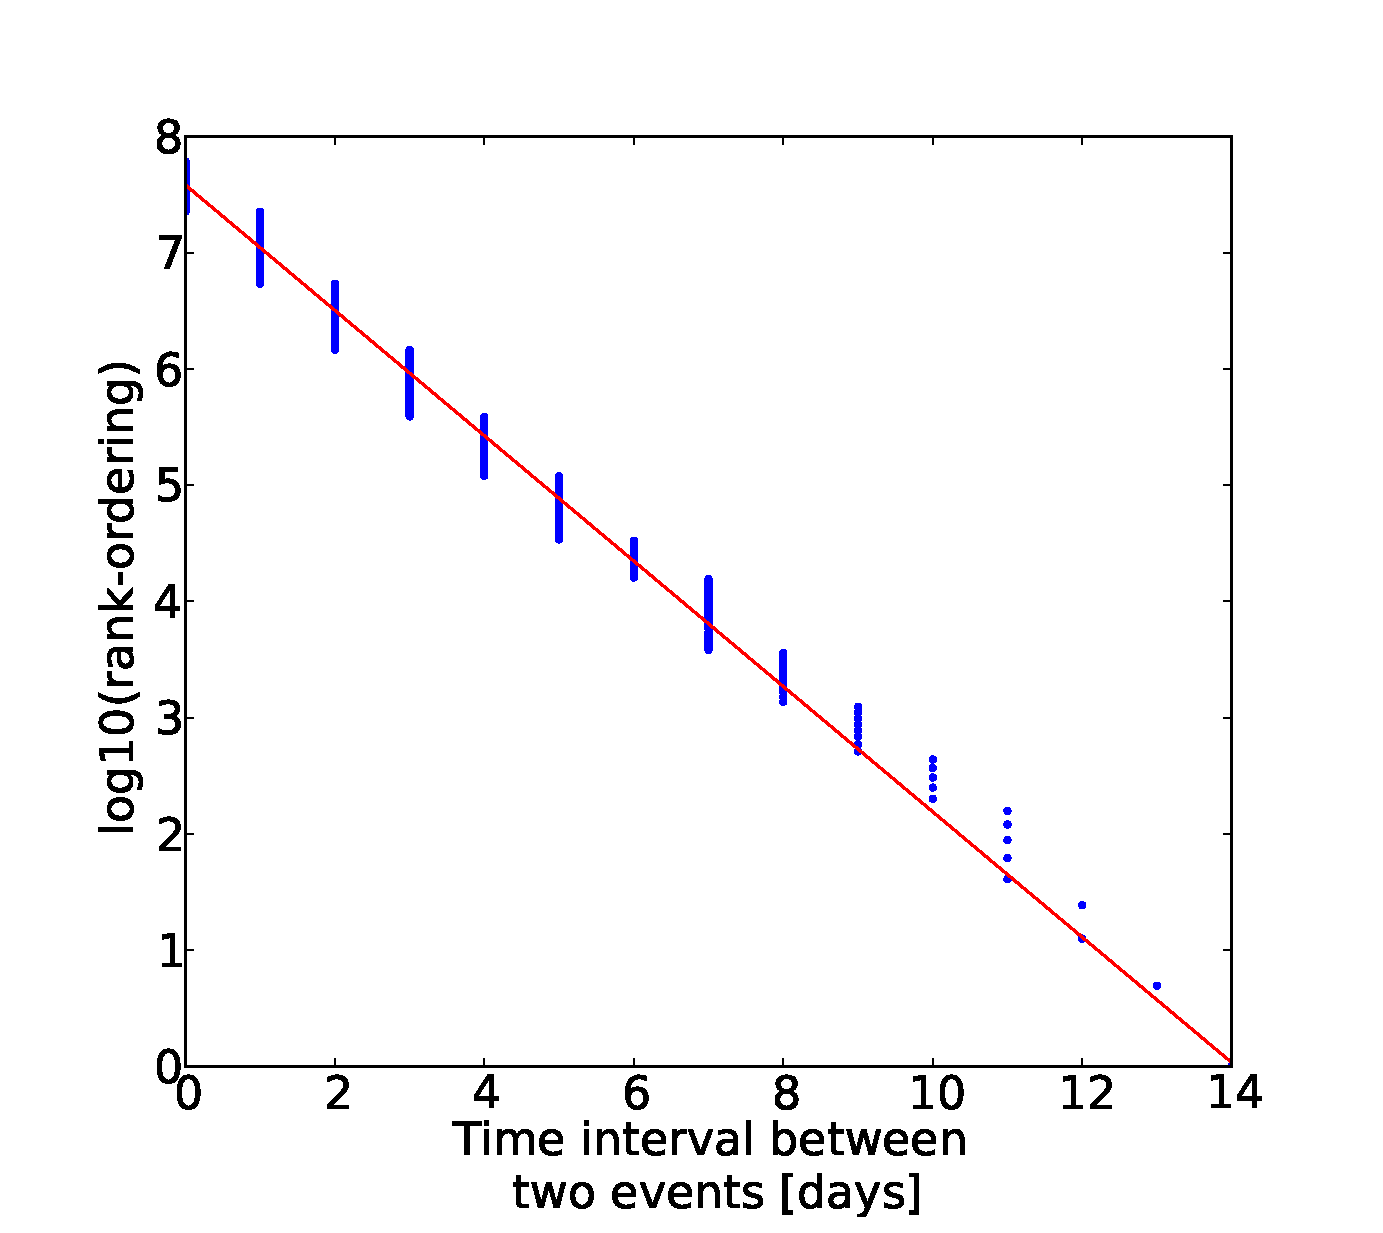
\includegraphics[width=4in]{../figures/SI/exponential_distribution.eps}
\caption{Distribution of rate of events of magnitude $M \geqslant 3.5$ and starting from 2005 ($t > 1825~days$). The straight line (red) in logarithmic y-scale and linear x-scale shows that the distribution of inter-time between two events is indeed exponential with $\lambda \approx 0.68$.}
\label{fig:exponential_rate}
\end{center}
\end{figure}




\begin{figure}[h]
\begin{center}
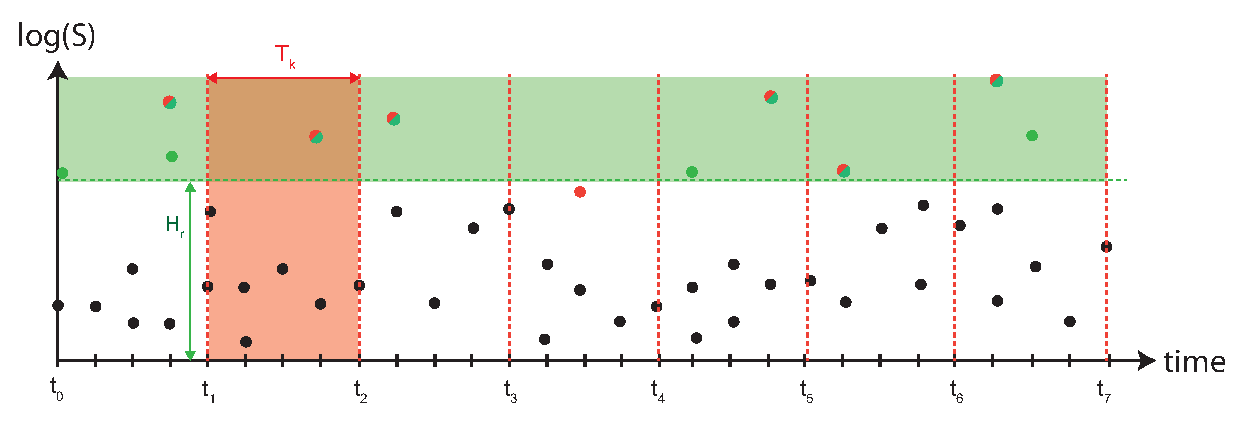
\includegraphics[width=6in]{../figures/SI/GEV_GPD_combined.eps}
\caption{Schematic of the combined GEV GPD method.}
\label{ }
\end{center}
\end{figure}






\subsection{Application of the GEV Method to the Data Breach catalog}


\subsection{Application of the GPD Method to the Data Breach catalog}

{\bf INSERT TABLE like {\it Table 18}}

\begin{enumerate}
  \item {\bf Choose the appropriate interval for T-values: } Kolmogorov distance + visual check ?
  \item 
  \item 
\end{enumerate}



